\documentclass[12pt]{article}

\usepackage[margin=0.5in]{geometry}
\usepackage{amsmath}
\usepackage{tikz}
\usepackage{soul}
\usepackage{hyperref}

\newcommand{\ds}{\displaystyle}

\begin{document}
\pagestyle{empty}
\subsubsection*{Midterm 3 Review Problems \hfill Math 141 }
\textit{These are suggested review problems similar to what might be on Midterm 3. Included with each problem is a link to a video where you can see how the problem is solved. I didn't make the videos, they are all  available on YouTube.}

\begin{enumerate}
\item Find the intervals of increase and decrease for the function $f(x) = \dfrac{x}{1+x^2}$.
\vfill 
\hfill  \url{https://youtu.be/oThEqQVHo9c} 
\hrule 

\item Find the intervals of concavity and inflection points for $f(x) = 6x^5 + x^4 - 5x -6$.
\vfill 
\hfill  \url{https://youtu.be/kivhvloJS7w} 
\hrule 

\item Find the following limits.
\begin{enumerate}
\item $\ds \lim_{x \rightarrow -\infty} \frac{5x-7x^3}{2x^2 + 14x^3 - 9}$. 
\vfill
\hfill \url{https://youtu.be/NmLljBAg82o?t=465}
\hrule

\item $\ds \lim_{x \rightarrow 0} \frac{\sin(7x)}{\sin(4x)}$. 
\vfill
\hfill \url{https://youtu.be/C-aFwHreB0U}
\end{enumerate}
\hrule


\newpage
\item A rectangular piece of cardboard is 20 inches by 30 inches.  If we cut a square from each corner of the cardboard and fold up the sides to make a box, how big should the squares be in order to maximize the volume?  
\begin{flushright}
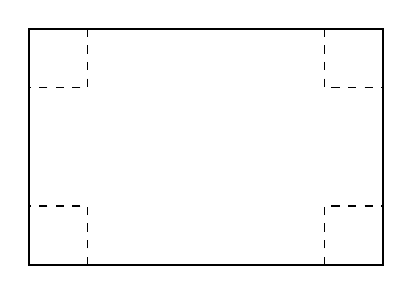
\begin{tikzpicture}[scale=1.5]
\draw[thick] (0,0) rectangle (3,2); 
\draw[dashed] (0.5,0) -- (0.5,0.5) -- (0,0.5);
\draw[dashed] (2.5,0) -- (2.5,0.5) -- (3,0.5);
\draw[dashed] (0.5,2) -- (0.5,1.5) -- (0,1.5);
\draw[dashed] (2.5,2) -- (2.5,1.5) -- (3,1.5);
\end{tikzpicture}
\end{flushright}
\vfill
\hfill \url{https://youtu.be/cRboY08YG8g}
\hrule

\item The hypotenuse of a right triangle is 20 centimeters long.  Find the value of the angle $\theta$ that maximizes the perimeter of the triangle. 
\begin{flushright}
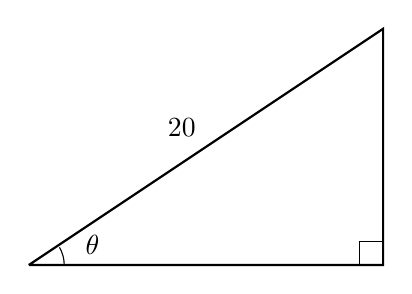
\begin{tikzpicture}[scale=1.5]
\draw[thick] (0,0) -- (3,0) -- (3,2) -- (1.5,1) node[above left] {$20$} -- (0,0); 
\draw (2.8,0) -- (2.8,0.2) -- (3,0.2);
\draw (0.3,0) arc(0:30:0.3);
\draw (0.54, 0.17) node {$\theta$};
\end{tikzpicture}
\end{flushright}
\vfill
\hfill \url{https://youtu.be/JjNpkQ_5tsY}
\hrule

%\item A ladder is positioned on the ground so that it leans against a vertical wall, and just clears a 2 meter tall fence that is one meter away from the wall (see picture). What is the minimum possible length of the ladder?
%\begin{flushright}
%\begin{tikzpicture}
%\fill[gray] (0,0) rectangle (-0.1,3);
%\draw[very thick] (-0.5,0) -- (0.5,0) node[below] {1} -- (6,0);
%\draw[very thick,red] (1,0) -- (1,1) node[right] {2} -- (1,2);
%\draw[very thick,blue] (0,2.5) -- (5,0);
%\draw (4.2, 0) arc(180:155:0.8);
%\draw (4.2,0.25) node[left] {$\theta$};
%\end{tikzpicture}
%\end{flushright}
%\vfill
%\hfill  \url{https://youtu.be/HdgZP3sfwuI} 
%\hrule 

%\item \hl{Something like this one again?} Suppose that $C(A)$ is the cost of building a house as a function of its area in square feet.  For each of the following equations, give a simple one sentence explanation (including units) of what exactly the equation is saying. 
%Or another optimization word problem?
%\begin{enumerate}
%\item $C(1{\small,}000) = 300{\small,}000$
%\item $C'(1{\small,}000) = 350$ 
%\end{enumerate}
%\vfill
%\hfill \url{https://youtu.be/QirtTPD0Unk?t=138}
%\hrule

\item Find $G(x)$ for $x > 0$, given that $G''(x) = 6x + \dfrac{5}{x^2}$, $G'(1) = 2$ and $G(1) = 3$. 
\vfill
\vfill
\hfill \url{https://youtu.be/n1fHUjHIgnk}
\hrule

\newpage
\item Calculate the following definite integrals.
\begin{enumerate}
\item $\ds \int_{-3}^5  4 \, dx$. 
\vfill
\hfill \url{https://youtu.be/auOcNZFKfo0}
\hrule

\item $\ds \int_{\tfrac{11\pi}{2}}^{6\pi}  9 \sin (x) \, dx$. 
\vfill
\hfill \url{https://youtu.be/ldLdWj6DLTw}
\hrule
\end{enumerate}


\item Find all antiderivatives of the following functions. 
\begin{enumerate}
\item $F'(x)= \tfrac{2}{3} x^{4/7}$. 
\vfill
\hfill \url{https://youtu.be/n0PeFRNAZ9c}
\hrule

\item $f(x) = \dfrac{x^4 - 2}{x^2}.$
\vfill
\hfill \url{https://youtu.be/PJFdN3E3mmo}
\hrule


\end{enumerate}
\end{enumerate}


\end{document}














